\chapter{Architektura systemu}

Ten rozdział opisuje architekturę systemu (rys. 3.1). Aplikacja będzie jednomodułowa. Składać się będzie z kilku warstw. Będą to:


\begin{enumerate}
    \item Warstwa prezentacji
    
    Ta warstwa odpowiedzialna będzie za wyświetlenie użytkownikowi elementów interfejsu użytkownika, takich jak ekran główny i ekran rozgrywki wraz z HUD.
    
    \item Warstwa logiki
    
    Ta warstwa odpowiedzialna będzie za obsługę logiki. Będzie ona odpowiadać za zmiany stanów obiektów oraz za obsługę zachowania obiektów fauny.
    
    \item Warstwa generatorów
    
    Ta warstwa odpowiedzialna będzie za tworzenie generowanej proceduralnie zawartości. Składać się będzie z mniejszych generatorów, które odpowiedzialne będą za generowanie terenu, roślinności i zwierząt.
\end{enumerate}

\begin{figure}[H]
    \centering
        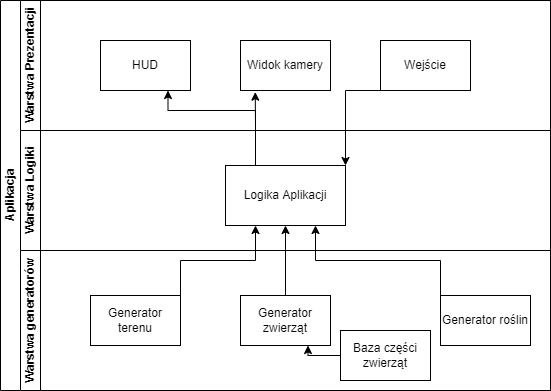
\includegraphics[width = 0.65\textwidth]{layers.png}
        \index{Diagram warstw aplikacji}
        \caption{Diagram warstw aplikacji}
\end{figure}